\documentclass[conference]{IEEEtran}
\IEEEoverridecommandlockouts
\usepackage{cite}
\usepackage{amsmath,amssymb,amsfonts}
\usepackage{graphicx}
\usepackage{textcomp}
\usepackage{xcolor}
\usepackage{booktabs}
\def\BibTeX{{\rm B\kern-.05em{\sc i\kern-.025em b}\kern-.08em
    T\kern-.1667em\lower.7ex\hbox{E}\kern-.125emX}}
\setcounter{dbltopnumber}{3}
\renewcommand{\dbltopfraction}{0.95}
\renewcommand{\textfraction}{0.05}
\renewcommand{\floatpagefraction}{0.85}
\begin{document}

\title{Multi-View VLM Verification for Semantic Object Extraction from a
Terrestrial Laser Scan Toward TOSM-Based Robot Environment Models}

\author{\IEEEauthorblockN{Sangmin Kim\IEEEauthorrefmark{1}\IEEEauthorrefmark{3},
Haryeong Kim\IEEEauthorrefmark{1},
Yonghyeon Song\IEEEauthorrefmark{1}\IEEEauthorrefmark{3},
Byeongjun Kim\IEEEauthorrefmark{2}\IEEEauthorrefmark{3}, and
Tae-Yong Kuc\IEEEauthorrefmark{1}\IEEEauthorrefmark{3}\thanks{Corresponding author: Tae-Yong Kuc (tykuc@skku.edu).}}
\IEEEauthorblockA{\IEEEauthorrefmark{1}Dept.\ of Electrical and Computer Engineering, Sungkyunkwan University, Suwon 16419, Republic of Korea\\
\IEEEauthorrefmark{2}Dept.\ of Intelligent Robotics, Sungkyunkwan University, Suwon 16419, Republic of Korea\\
\IEEEauthorrefmark{3}CASELab Co., Ltd., Anyang 14118, Republic of Korea\\
kimsang.m@g.skku.edu, khy0403@skku.edu, songyong2535@g.skku.edu, byeongjunkim@g.skku.edu, tykuc@skku.edu}
}

\maketitle

\begin{abstract}
Semantic environment models such as the Triplet Ontological Semantic Model
(TOSM) give indoor mobile robots the symbolic, explicit, and implicit
knowledge needed for task-level autonomy, but populating them for an
existing facility is still manual work. This paper presents an automated
pipeline that extracts TOSM semantic objects from a single terrestrial
laser scan and emits them as a VDA~5050-style JSON message. A deterministic
stage segments the colored point cloud and fills the explicit model (pose,
dimensions, color) with a provisional class from an open-vocabulary 3D
classifier; a vision--language model (VLM) stage then verifies each class
from multi-view object renders under forced tool-use and infers the
implicit affordance model. We show that the obvious multi-view strategy ---
feeding all views into one prompt (early fusion) --- \emph{degrades}
accuracy on sparse point renders, and propose per-view classification with
confidence-weighted voting (late fusion) instead. On a 68.5M-point scan of
a robot showroom (57 objects), late fusion cuts wrong labels from 24
(classifier-only) to 15 and is the strongest multi-view strategy (74\% vs.\
67\% lenient accuracy over early fusion), while providing a free
reliability signal: label votes unanimous across views are 94\% correct,
against 30\% for split votes --- gating validated when an on-site
inventory check overturned a label that had fooled both the VLM and the
human audit. Full-scene verification costs \$2.6.
\end{abstract}

\begin{IEEEkeywords}
multi-view object recognition, vision--language model, semantic mapping,
terrestrial laser scanning, TOSM, VDA 5050
\end{IEEEkeywords}

\section{Introduction}
Task-level autonomy for indoor mobile robots requires more than an
occupancy grid: the robot must know \emph{what} objects occupy the space,
\emph{where} they are, and \emph{how} they can be interacted with. The
Triplet Ontological Semantic Model (TOSM)~\cite{joo2020tosm} organizes this
knowledge into a \emph{symbolic} model (class, name, identity), an
\emph{explicit} model (pose, size, color), and an \emph{implicit} model
(affordances such as whether an object is a reliable landmark or can be
displaced). TOSM-style databases drive navigation frameworks and multi-robot
fleets, and their content maps naturally onto the JSON message conventions
of VDA~5050~\cite{vda5050}, the emerging interface standard between AGV
fleets and master control systems.

In practice, the semantic-object database for a new facility is authored by
hand. Terrestrial laser scanners (TLS) such as the Leica BLK360 capture a
dense, colored as-built model in minutes, and scan-to-BIM
research~\cite{patraucean2015} recovers structural geometry automatically,
but object-level semantics remain the gap: open-vocabulary 3D classifiers
such as Uni3D~\cite{zhou2024uni3d} are biased toward industrial structural
classes --- in our experiments office chairs were labeled \emph{stair} or
\emph{machine} and displays \emph{ladder} --- and no point-cloud classifier
produces the affordance-level knowledge TOSM needs.

Vision--language models (VLMs) offer a complementary signal: rendered views
of a segmented object carry texture and context that a point-cloud embedding
discards. Since multi-view recognition classically outperforms single-view,
we render each object from four azimuths and study how a VLM should consume
them. The naive strategy --- all views in one prompt (\emph{early fusion})
--- turns out to \emph{hurt}: sparse oblique point renders invite
over-confident misreadings that contaminate the joint judgment. Classifying
each view independently and aggregating by confidence-weighted vote
(\emph{late fusion}), the multi-view analogue of MVCNN-style
aggregation~\cite{su2015mvcnn}, recovers most of the lost reliability and
exposes disagreement between views as an explicit uncertainty signal. The contributions are:

\begin{itemize}
\item an automated TLS-to-TOSM pipeline whose output is a VDA~5050-style
      \texttt{semanticObjects} message consumable by a fleet environment
      model;
\item a schema-forced VLM verification protocol with per-view late fusion,
      plus prompt guardrails (size sanity, sparse-render caution, panel
      disambiguation) for point-render inputs;
\item a six-configuration study on a real 68.5M-point BLK360 scan (57
      objects) with a consistent, inventory-checked manual audit, showing
      early fusion degrades accuracy, late fusion is the strongest
      multi-view strategy, and vote unanimity yields 94\%-precise gating.
\end{itemize}

\begin{figure}[t]
\centering
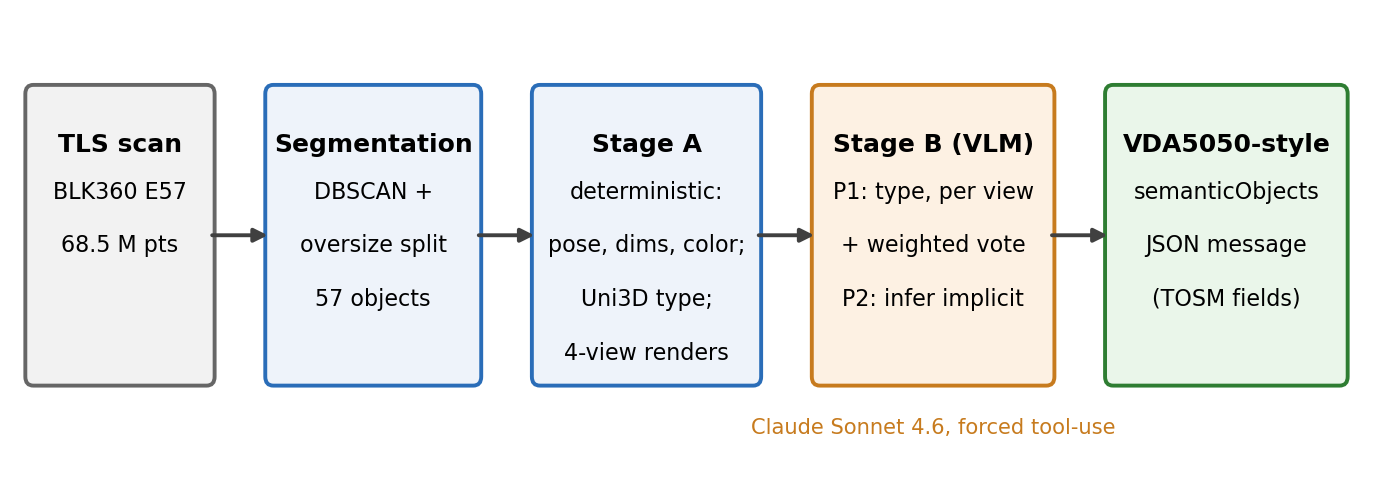
\includegraphics[width=0.86\columnwidth]{fig_pipeline.png}
\caption{Scan-to-semantics pipeline. Stage A deterministically fills the
explicit TOSM model plus a provisional class; Stage B verifies the symbolic
model per view with weighted late fusion and infers the implicit model.}
\label{fig:pipeline}
\end{figure}

\section{Related Work}
\textbf{Semantic environment models.} TOSM~\cite{joo2020tosm} extends
ontology-based robot knowledge bases~\cite{tenorth2013} with the
symbolic/explicit/implicit triplet; its records subsume the object fields of
VDA~5050~\cite{vda5050} messages, which we adopt as the output container;
the taxonomy also underpins a knowledge-grounded 3D scene graph for LLM
querying~\cite{kim2025isis}, whose records we populate automatically.
\textbf{Scan-to-model.} As-built modeling from TLS has focused on
structural elements~\cite{patraucean2015}; object semantics are left to
learned 3D segmentation~\cite{qi2017} or open-vocabulary encoders such as
Uni3D~\cite{zhou2024uni3d}, which inherit training-corpus biases.
\textbf{Multi-view recognition.} Aggregating rendered views is a classic
route to 3D shape recognition (MVCNN~\cite{su2015mvcnn}); we revisit the
early-vs-late fusion question for VLM prompts over \emph{sparse point}
renders rather than mesh renders. \textbf{VLMs in robotics.} Recent systems
use VLMs for open-set scene graphs~\cite{gu2024conceptgraphs} and
language-driven maps~\cite{huang2023vlmaps}. We use a VLM in a narrower,
auditable role: verifying one object at a time against measured geometry.

\section{Pipeline}

\subsection{Stage A: Deterministic Explicit Model}
The input is a single registered BLK360 scan (E57, colored). After floor
detection by RANSAC and wall removal, objects are segmented by DBSCAN~\cite{ester1996} with a
conservative re-clustering pass that splits clusters whose footprint exceeds
2.5\,m (30$\rightarrow$57 objects on our scene). Segmentation stays
geometric because ScanNet-trained instance segmenters did not transfer to
this industrial scene: on the same cloud, SPFormer assigned only 51\% of
points with furniture-biased labels, and PTv3 labeled 46\% of points
\emph{wall} even after wall removal. For each object Stage~A
computes the explicit TOSM model directly from the points: bounding-box
center (\texttt{poseX/Y}, \texttt{properties.poseZ}), PCA-based yaw
(\texttt{poseTheta}), yaw-aligned extents (\texttt{dimensions}), and a mean
RGB color name. Uni3D provides a \emph{provisional} symbolic class, and four
azimuth renders (0/90/180/270$^{\circ}$, 512$\times$512, point size~8, red
3D bounding box) are exported; smaller point sizes produced speckle-like
views that misled both the VLM and the human auditors
(Sec.~\ref{sec:study}). All Stage-A fields are measured, not generated;
Stage~B never modifies them.

\subsection{Stage B: VLM Verification with Late Fusion}
\label{sec:stageb}
Stage B calls a commercial VLM (Claude Sonnet 4.6) with \emph{forced
tool-use}: the model must answer by calling a declared JSON tool, so every
response is schema-valid by construction. Fig.~\ref{fig:prompt} condenses
the prompt design.

\emph{Prompt 1 (symbolic), once per view.} The VLM sees ONE render, the
measured dimensions, the provisional class, and an optional candidate
vocabulary (\emph{chair, TV, monitor, Mobile Robot, desk}). The decision
rule is three-way: keep a correct label; if wrong, prefer a fitting
candidate; else emit an open-vocabulary label. Guardrails address
point-render failure modes (Fig.~\ref{fig:prompt}): dimensions as a hard
constraint, oversize clusters treated as merged objects, thin-panel
disambiguation, a ban on claiming parts not outlined by points, and a
keep-or-\emph{clutter} fallback when no label is clearly supported.

\emph{Late fusion.} The four per-view reports are aggregated by
confidence-weighted voting: each vote adds its confidence to its label's
score, the top-scoring label wins, and the final confidence is the winner's
share of the total. The per-view votes are stored in the record
(\texttt{properties.viewVotes}), so a downstream consumer can distinguish a
4/4 unanimous label from a 2/4 split --- an uncertainty signal that costs
nothing extra. Fig.~\ref{fig:votes} shows a unanimous case: all four
azimuths of a robot manipulator agree independently, giving fused
confidence 1.0. Conversely, a single contaminated view is simply outvoted
(a tall-backed chair whose frontal view read \emph{Mobile Robot} fused to
\emph{chair} 3:1), whereas the same view inside one early-fusion prompt
can drag the joint judgment toward the wrong label.

\begin{figure}[t]
\centering
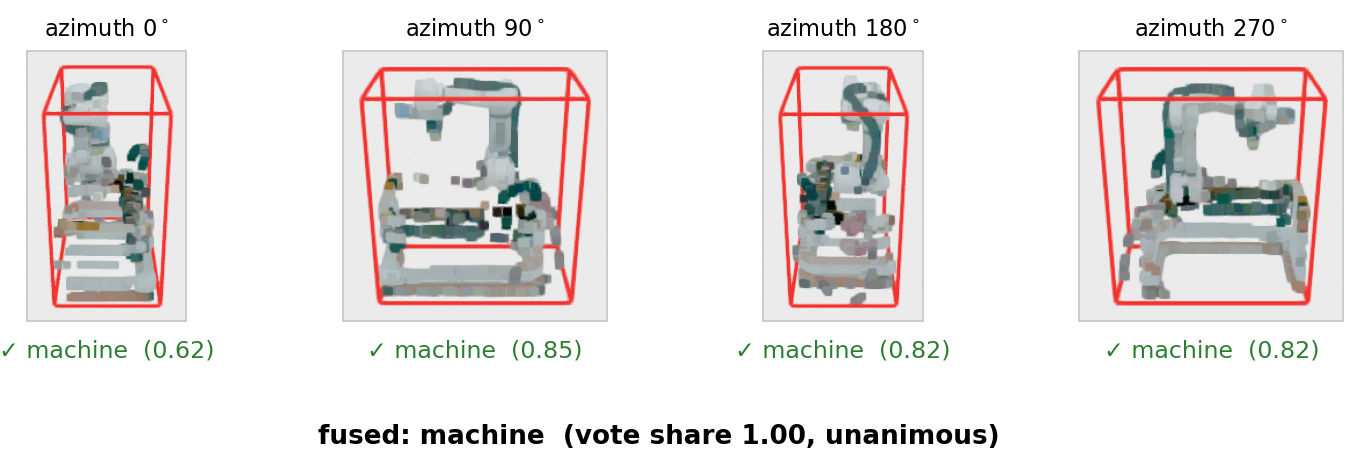
\includegraphics[width=0.74\columnwidth]{fig_votes.png}
\caption{Late fusion on one object (\texttt{machine\_004}). Each of the
four azimuth renders is classified independently; here all views agree,
yielding the unanimous, confidence-1.0 case that our audit finds 94\%
reliable (Sec.~\ref{sec:study}).}
\label{fig:votes}
\end{figure}

\emph{Prompt 2 (implicit), once per object.} Given the fused type and all
views, the VLM reports the TOSM implicit model: \texttt{isKeyObject},
\texttt{isMovable}, and (doors only) \texttt{isOpen}/\texttt{canBeOpen}.

\begin{figure}[t]
\centering
\fbox{\begin{minipage}{0.94\columnwidth}\footnotesize
\textbf{P1 system (condensed).} You are a semantic-mapping verifier for an
indoor mobile robot. You see a render of ONE segmented 3D object (sparse
laser points, red 3D box), its classifier label \texttt{uni3d\_type}, and
optional candidates. \emph{Decision rule:} (1)~if \texttt{uni3d\_type} is
correct, KEEP; (2)~if wrong, replace --- (a)~prefer a fitting candidate,
(b)~else the most accurate common-noun label. Never `unknown'.
\emph{Size sanity:} measured dimensions are a HARD constraint; a cluster
exceeding a class's envelope is merged objects --- label the dominant
structure or `clutter'. \emph{Sparse-render caution:} never claim parts not
clearly outlined by points. \emph{Panel rule:} thin flat objects are
keyboard (key grid) / display (uniform dark face) / shelf --- never ladder.
\emph{Chair gate:} requires visible seat pan 0.3--0.6\,m high plus
backrest. If uncertain, keep a size-compatible label. Respond ONLY via the
\texttt{report\_symbolic} tool.\\[2pt]
\textbf{P2 system (condensed).} Infer implicit properties of ONE object
from its views and confirmed type: \texttt{isKeyObject} (fixed, distinctive
landmark), \texttt{isMovable}, \texttt{isOpen}/\texttt{canBeOpen} (doors
only, else null). Respond ONLY via the \texttt{report\_implicit} tool.
\end{minipage}}
\caption{Condensed Stage-B prompt design. Forced tool-use makes every
response schema-valid JSON; measured geometry is read-only context.}
\label{fig:prompt}
\end{figure}

\subsection{TOSM to VDA 5050-Style Message}
The completed records are serialized as one \texttt{semanticObjects} JSON
message with a VDA~5050-style header. Table~\ref{tab:mapping} shows the
field mapping; TOSM fields with no standard slot travel in the extensible
\texttt{properties} map, so the message remains readable by consumers that
only know the base schema.

\begin{table}[t]
\caption{TOSM $\rightarrow$ VDA 5050-style JSON field mapping}
\label{tab:mapping}
\centering
\scriptsize
\begin{tabular}{@{}lll@{}}
\toprule
TOSM model & element & JSON field \\
\midrule
symbolic & class & \texttt{type} \\
         & name / identity & \texttt{name}, \texttt{id} \\
explicit & position $(x,y)$ & \texttt{poseX}, \texttt{poseY} \\
         & height $z$ & \texttt{properties.poseZ} \\
         & orientation & \texttt{poseTheta} \\
         & size & \texttt{dimensions\{l,w,h\}} \\
         & color & \texttt{color} \\
implicit & landmark / movability & \texttt{properties.isKeyObject,} \\
         & door state & \texttt{isMovable, isOpen, canBeOpen} \\
--       & VLM audit trail & \texttt{properties.viewVotes,} \\
         &                 & \texttt{symbolicReason, confidence} \\
\bottomrule
\end{tabular}
\end{table}

\section{Experiments}

\subsection{Setup and Audit Protocol}
We evaluate on a single BLK360 scan of an indoor robot showroom (68.5M
colored points, 57 segmented objects) with Claude Sonnet 4.6. Six
configurations are compared (Table~\ref{tab:configs}): the classifier
alone; single-view and four-view early-fusion prompts, each with the
initial sparse renders/base prompt and with dense renders/guardrail prompt;
and four-view late fusion. To grade them consistently, two of the authors
audited all 57 objects against the \emph{dense} four-view renders and the
measured dimensions, rating every configuration's final label
\emph{correct}, \emph{plausible} (consistent with the views but not
verifiable from renders alone), or \emph{wrong}. Metered cost: late fusion
\$2.63 per scene (285 calls, \$0.046/object); early fusion \$1.27; single
view \$0.87.

\subsection{Multi-View Study}
\label{sec:study}
Table~\ref{tab:configs} and Fig.~\ref{fig:accuracy}(b) summarize the
audit. Three findings stand out.

\emph{(1) Early fusion hurts.} Feeding four sparse views into one prompt
dropped strict accuracy from 60\% (single view) to 49\%: extra oblique
speckle views encouraged over-committed readings, e.g.\ two electrical
cabinets confidently relabeled \emph{chair}. Denser renders and the prompt
guardrails did not close the gap (46\% vs.\ 51\%).

\emph{(2) Late fusion is the strongest multi-view strategy.} Judging each
view independently and voting beats early fusion on every measure (15 vs.\
19 wrong labels, 74\% vs.\ 67\% lenient): a contaminated view can no
longer dominate --- it is outvoted. It does not, however, overtake the best
single canonical view (60\%/81\%): on sparse point clouds, extra views
add noise faster than evidence unless aggregation is vote-based. The cost
of voting is a larger \emph{plausible} bucket --- split votes often land
on \emph{clutter} --- trading decisiveness for safety, the right trade for
an autonomously written robot database.

\emph{(3) Vote unanimity is a free precision signal.} 17 of 57 objects
received identical labels from all four views; 16 of those (94\%) were
audited correct, versus 30\% among split-vote objects. Gating on the stored
\texttt{viewVotes} thus gives a downstream consumer a calibrated
route-to-human-review policy that per-call confidence alone did not
provide.

Render density cut both ways, and produced the study's starkest warning:
dense renders made four dotted-grid panels look so convincingly like
keyboards (per-view confidence up to 0.97) that the label passed our
render-based audit --- only the facility owner's inventory check revealed
it was wrong, and Table~\ref{tab:configs} grades every such label wrong.
The incident is the strongest argument for the gating above: a label that
fools both the VLM and a human at the same renders was still caught by
vote splits (these objects never reached unanimity). Run-to-run sampling
variance ($\pm$2--3 objects) bounds how finely the configurations can be
ranked.

\begin{table}[t]
\caption{Manual audit of final type labels (57 objects). C/P/W = correct /
plausible / wrong; strict = C, lenient = C+P.}
\label{tab:configs}
\centering
\footnotesize
\begin{tabular}{@{}lccccc@{}}
\toprule
Configuration & C & P & W & strict & lenient \\
\midrule
Uni3D only (no VLM)            & 28 & 5  & 24 & 49\% & 58\% \\
1 view, base prompt, sparse    & 34 & 12 & 11 & 60\% & 81\% \\
4 views early fus., sparse     & 28 & 10 & 19 & 49\% & 67\% \\
1 view, guardrails, dense      & 29 & 11 & 17 & 51\% & 70\% \\
4 views early fus., dense      & 26 & 12 & 19 & 46\% & 67\% \\
\textbf{4 views late fus., dense} & \textbf{28} & \textbf{14} & \textbf{15}
  & \textbf{49\%} & \textbf{74\%} \\
\bottomrule
\end{tabular}
\end{table}

\begin{figure}[t]
\centering
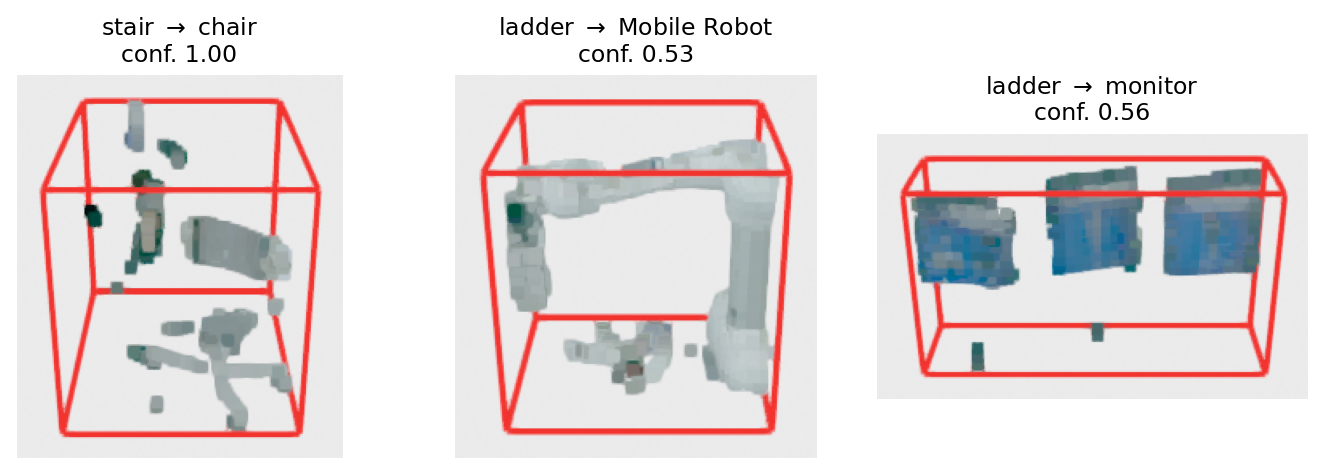
\includegraphics[width=0.58\columnwidth]{fig_examples.png}
\caption{Representative late-fusion corrections (one of four dense views;
provisional label $\rightarrow$ fused label, vote-share confidence). The 3D
classifier's industrial bias (\emph{stair}, \emph{ladder}) is corrected to
furniture, robots, and displays; the chair correction is detailed
view-by-view in Fig.~\ref{fig:votes}.}
\label{fig:examples}
\end{figure}

\begin{figure*}[t]
\centering

\includegraphics[width=0.62\textwidth]{fig_accuracy.png}
\caption{Effect of VLM verification on the 57-object scene. (a)~Class
distribution, classifier-only vs.\ after late fusion: implausible
\emph{ladder}/\emph{stair} populations are redistributed to displays and
furniture (the keyboard outputs were later rejected by the on-site
inventory, Sec.~\ref{sec:study}). (b)~Manual audit: early fusion degrades
single-view accuracy; late fusion is the strongest multi-view strategy (15
wrong labels vs.\ 19 for early fusion).}
\label{fig:accuracy}
\end{figure*}

\begin{figure*}[!t]
\centering
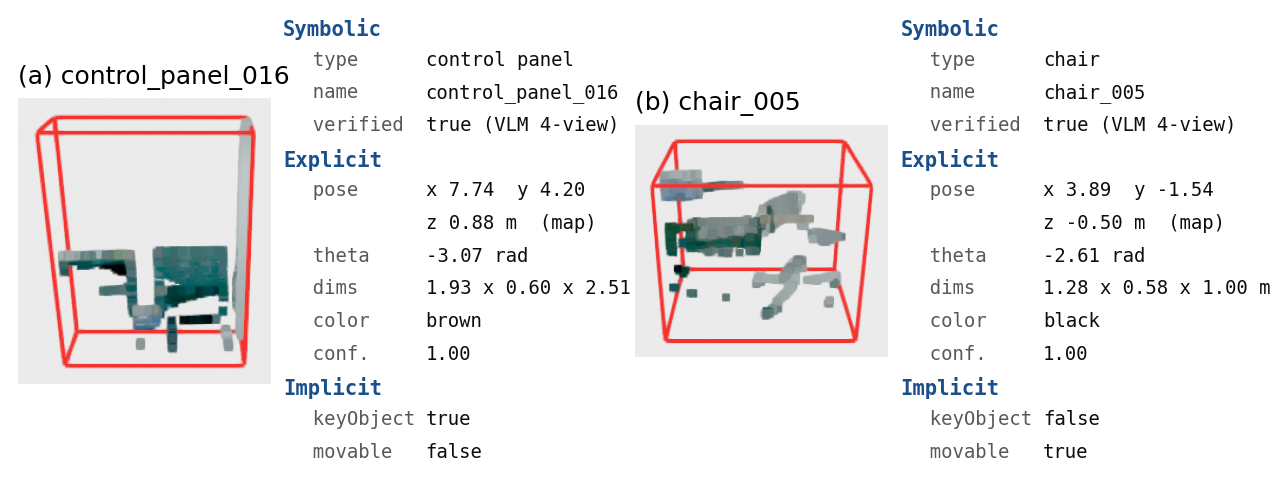
\includegraphics[width=0.62\textwidth]{fig_cards.png}
\caption{Completed TOSM semantic-object records (dense render + symbolic /
explicit / implicit fields) as serialized into the VDA 5050-style message.
(a)~A control panel, unanimously verified and marked as a fixed key
landmark. (b)~An office chair corrected from \emph{stair}, movable and not
a landmark.}
\label{fig:cards}
\end{figure*}

\subsection{Implicit Model and Completed Records}
On the late-fusion output, Prompt 2 marked 6 of 57 objects as key objects
(control panels, a large machine, mobile robots, a wall display) and 50 as
movable. Fig.~\ref{fig:cards} shows two completed TOSM records as stored in
the output message, including the audit trail (per-view votes, fused
confidence, one-sentence reason). Mean fused confidence was 0.71, and the
17 unanimous objects carry confidence 1.0 by construction, aligning the
stored confidence with the observed 94\% unanimity precision. By design
the generated records are a reviewable draft, not ground truth: the
semantic model remains user-editable and every amendment is logged in the
record's audit trail. An owner review exercised exactly this loop on the
implicit model, correcting two movability entries (a wheeled machine
judged fixed, a wall-mounted display judged movable) at negligible cost.

\subsection{Discussion and Limitations}
The division of labor is the main design point: everything measurable stays
deterministic and VLM-immutable, so hallucination can corrupt neither poses
nor dimensions, and the VLM contributes exactly the judgments geometry
cannot make --- naming and affordances --- in an auditable form (per-view
votes, forced-tool JSON, stored reasons). All 741 tool calls
across the five VLM configurations returned schema-valid
JSON. Remaining errors concentrate where the render itself is ambiguous
(texture-poor slabs, merged clusters, sparse strips), pointing to upstream
fixes --- finer segmentation, mesh renders --- not to the fusion protocol.
Absolute strict accuracy ($\sim$49--60\%) reflects a deliberately hard
test bed: a cluttered showroom scanned once, without manual cleanup.

\section{Conclusion}
We presented an automated pipeline that turns a single terrestrial laser
scan into TOSM semantic-object records delivered as a VDA 5050-style JSON
message, using a VLM in a tightly scoped, schema-forced role. A
six-configuration study showed that the intuitive multi-view prompt ---
all views at once --- degrades verification on sparse point renders,
whereas per-view classification with confidence-weighted late fusion is the
strongest multi-view strategy: wrong labels drop from 24 (classifier-only)
to 15, lenient accuracy reaches 74\%, and vote unanimity provides a
94\%-precise gating signal at \$2.6 per scene. Future work includes
mesh-based renders, finer segmentation, and coupling the records to place
modeling and a live digital twin.

\begin{thebibliography}{00}
\bibitem{joo2020tosm} S.-H. Joo \emph{et al.}, ``Autonomous navigation
framework for intelligent robots based on a semantic environment modeling,''
\emph{Applied Sciences}, vol.~10, no.~9, p.~3219, 2020.
\bibitem{vda5050} VDA and VDMA, ``VDA 5050: Interface for the communication
between automated guided vehicles (AGV) and a master control,'' ver.~2.0,
2022.
\bibitem{patraucean2015} V. P\u{a}tr\u{a}ucean, I. Armeni, M. Nahangi,
J. Yeung, I. Brilakis, and C. Haas, ``State of research in automatic
as-built modelling,'' \emph{Adv. Eng. Informat.}, vol.~29, no.~2,
pp.~162--171, 2015.
\bibitem{zhou2024uni3d} J. Zhou, J. Wang, B. Ma, Y.-S. Liu, T. Huang, and
X. Wang, ``Uni3D: Exploring unified 3D representation at scale,'' in
\emph{Proc. Int. Conf. Learn. Represent. (ICLR)}, 2024.
\bibitem{su2015mvcnn} H. Su, S. Maji, E. Kalogerakis, and E.
Learned-Miller, ``Multi-view convolutional neural networks for 3D shape
recognition,'' in \emph{Proc. IEEE Int. Conf. Comput. Vis. (ICCV)}, 2015,
pp.~945--953.
\bibitem{tenorth2013} M. Tenorth and M. Beetz, ``KnowRob: A knowledge
processing infrastructure for cognition-enabled robots,'' \emph{Int. J.
Robot. Res.}, vol.~32, no.~5, pp.~566--590, 2013.
\bibitem{kim2025isis} H. Kim, K. Joo, G. Galvis Giraldo, S. Kim, and
T.-Y. Kuc, ``Toward long-term memory in embodied AI: A knowledge-grounded
3D scene graph framework,'' in \emph{Proc. 26th Int. Symp. Adv. Intell.
Syst. (ISIS)}, Cheongju, Korea, 2025, pp. 237--240.
\bibitem{qi2017} C. R. Qi, H. Su, K. Mo, and L. J. Guibas, ``PointNet: Deep
learning on point sets for 3D classification and segmentation,'' in
\emph{Proc. IEEE Conf. Comput. Vis. Pattern Recognit. (CVPR)}, 2017,
pp.~652--660.
\bibitem{gu2024conceptgraphs} Q. Gu \emph{et al.}, ``ConceptGraphs:
Open-vocabulary 3D scene graphs for perception and planning,'' in
\emph{Proc. IEEE Int. Conf. Robot. Autom. (ICRA)}, 2024, pp.~5021--5028.
\bibitem{huang2023vlmaps} C. Huang, O. Mees, A. Zeng, and W. Burgard,
``Visual language maps for robot navigation,'' in \emph{Proc. IEEE Int.
Conf. Robot. Autom. (ICRA)}, 2023, pp.~10608--10615.
\bibitem{ester1996} M. Ester, H.-P. Kriegel, J. Sander, and X. Xu, ``A
density-based algorithm for discovering clusters in large spatial databases
with noise,'' in \emph{Proc. 2nd Int. Conf. Knowl. Discov. Data Min.
(KDD)}, 1996, pp. 226--231.
\end{thebibliography}

\end{document}
